\documentclass[12pt,a4paper]{book}
\usepackage[utf8]{inputenc}
\usepackage[english]{babel}
\usepackage{amsmath}
\usepackage{amsfonts}
\usepackage{amssymb}
\usepackage{graphicx}
\usepackage{wrapfig}
\usepackage{subcaption}
\usepackage[left=2cm,right=2cm,top=2cm,bottom=2cm]{geometry}
\usepackage{siunitx}

% Nice captions.
\usepackage[format=hang,font=small,labelfont=bf]{caption}
\setlength{\captionmargin}{25pt}

% define the symbols := and =: for ease of use
\usepackage{mathtools}
\newcommand{\defeq}{\vcentcolon=}
\newcommand{\eqdef}{=\vcentcolon}
    
% define bra and ket
\newcommand{\bra}[1]{%
	\left\langle #1 \right|
}
\newcommand{\ket}[1]{%
	\left| #1 \right\rangle
}
\newcommand{\bracket}[2]{%
	\left\langle #1 | #2 \right\rangle
}

% multiline commenting \begin{comment}
\usepackage{comment}
% package to cancel obliquely symbols
\usepackage{cancel}

% generate correct 1-bold (identity operator) font
\usepackage{dsfont}
% generate correct bold greek letters
\usepackage{bm}
% to produce stroked integral \fint
\usepackage{esint}

% better boxes (also multiple equations)
\usepackage{tcolorbox}
\tcbuselibrary{theorems}

% author managing package
\usepackage{authblk}

\title{Photonic Artificial Neural Networks}
\author[]{Davide Bazzanella}
\affil[]{Department of Physics, University of Trento}

% to create an index with terms and the corresponding page(s)
\usepackage{makeidx}
\makeindex

% create plots
\usepackage{pgfplots} % README here http://pgfplots.sourceforge.net/pgfplots.pdf
\pgfplotsset{compat=1.14} 	%ShareLaTeX wants \pgfplotsset{compat=1.14}

% externalize tikz images
\usepackage{tikz}
\usetikzlibrary{external}
\tikzexternalize[prefix=tikz/] % activate!

% draws bloch sphere
%\usepackage{blochsphere}

\begin{document}

% need this to fill between functions
\usepgfplotslibrary{fillbetween}
\usetikzlibrary{patterns,decorations,arrows, shapes.geometric}
\usetikzlibrary{arrows.meta}

% define the box around functions
\newtcolorbox{mymathbox}[1][]{colback=white, sharp corners, #1}

\maketitle
\tableofcontents
%\cleardoublepage
\clearpage

\chapter{Introduction}
WHAT and WHY?
BACKUP project, why silicon photonics (CMOS compatibility)

\chapter{Artificial Neural Networks}
THEORY ON ANNs
Artificial Neural Networks (ANNs) are computing devices which operate in way that mimics biological neural networks.
\section{Types of ANNs}
\subsection{Feed Forward NN}
\subsubsection{FF NN node}
%\begin{wrapfigure}[5]{r}{0.4\textwidth}
\begin{figure}[ht]
	\centering
	\begin{tikzpicture}
		\node [shape=circle, minimum size=2cm, draw=gray!100, fill=gray!20]%
					(af) at (1.5,0) {\LARGE $f_a$};
		\node at (af.south) [below, align=center] {activation \\ function};
		\node [regular polygon, regular polygon sides=6, minimum size=2cm, draw=gray!100, fill=gray!20]%
					(ws) at (-2,0) {\LARGE $\Sigma$};
		\node at (ws.south) [below, align=center] {weighted \\ sum};
		\draw (ws) to (af);
		\foreach \i in {1,2,4}	\draw (-4.5,1.5-0.6*\i) .. controls (-3.5,1.5-0.6*\i) .. (ws);
		\draw [dashed] (-4.5,-0.3) node {$\vdots\qquad$} .. controls (-3.5,-0.3) .. (ws);
		\foreach \i in {1,2}		\node at (-4.5,1.5-0.6*\i) [left] {$x_\i$};
		\node at (-4.5,-0.9)  [left] {$x_n$};
		\draw (-2,1.5) node [above] {$w_0$} to (ws);
		\draw (af) to (3.5,0) node [right] {$y$};
	\end{tikzpicture}
	\caption{Feed Forward node}
	\label{fig:FF_node}
\end{figure}
%\end{wrapfigure}
\begin{equation}
y = f_a \left(  w_0 + \sum_i^n w_i x_i \right)
\label{eq:node_function}
\end{equation}
\subsection{Other Types of ANNs}

\chapter{Photonics applied to ANNs}
How do I intend to create a hardware photonic ANN node?
\section{Weighted sum of inputs}
This thing has already been demonstrated and integrated widely, so it will not be the focus of this work.
\section{Nonlinear activation function}
On the other hand, a photonic nonlinear activation function has not yet been found.
This is where the focus of my work will be.

\subsection{Simulations}

\chapter{Samples, setup and measurements}
\section{The samples}
I could say that in the time this work was done there would have not been enough time to design and produce an ad hoc device. The aim of this thesis is to produce a proof of concept, to answer the question of feasibility.
\vspace{1em}

The samples on which this work is based have been provided by the IRIS project.
Specifically I had a few different structures available: from single rings resonators to the full matrix, each accessible via grating couplers.
My choice was a system of intermediate complexity: a simple waveguide, coupled to eight drop channels by a single or a couple of ring resonators each.
Moreover, these samples were provided with thermo-electric pads to heat the rings and effectively tune their resonance.
The final choice was to study the \textit{mini-matrix} in which the coupling mechanism was provided by single ring resonators, because it was considered simpler.

\begin{figure}[ht]
	\centering
	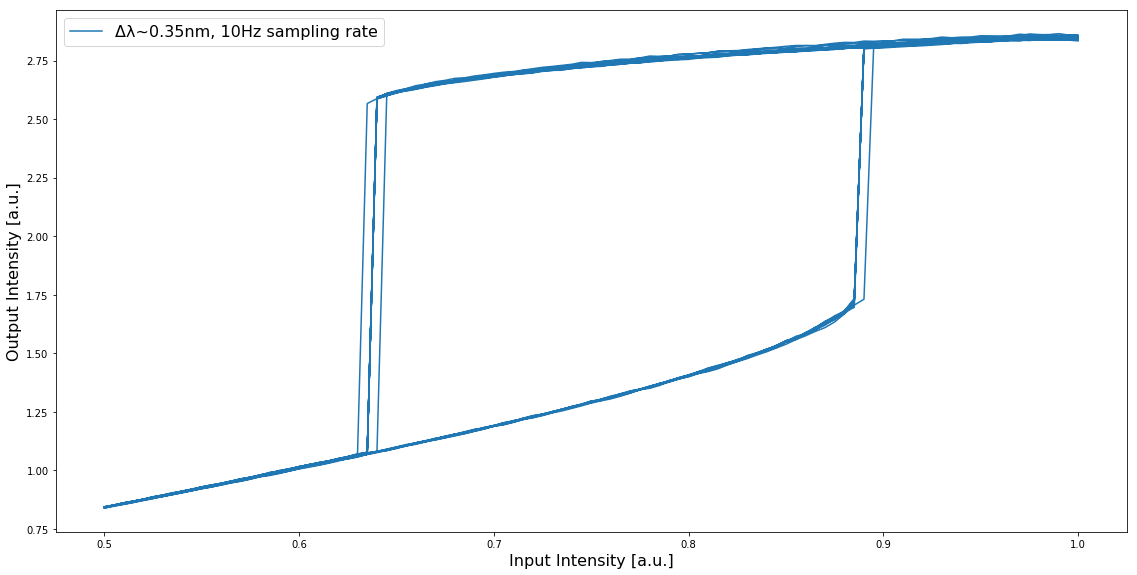
\includegraphics[draft,width=9cm,height=6cm]{figures/foo.png}
	\caption{image/scheme of the minimatrix}
	\label{fig:minimatrix_full}
\end{figure}



\end{document}